\documentclass[unicode]{article}

\usepackage[utf8]{inputenc}
\usepackage{standalone}
\usepackage{color}
\usepackage{amsmath}
\usepackage{graphics}
\usepackage[colorlinks,urlcolor=blue]{hyperref}
\usepackage{tikz}
\usepackage{tikz-3dplot}
\usetikzlibrary{decorations.pathreplacing,calligraphy}

\textheight=26cm 
\textwidth=18cm
\oddsidemargin=-1cm
\topmargin=-2.5cm

\newcommand{\pmat}[1]{\begin{pmatrix}#1\end{pmatrix}}

\begin{document}

\section{Classic Cart Pole}

\subsection{Dynamic}

\begin{center}
    \documentclass[dvisvgm,tikz]{standalone}

\usepackage{tikz}

\begin{document}
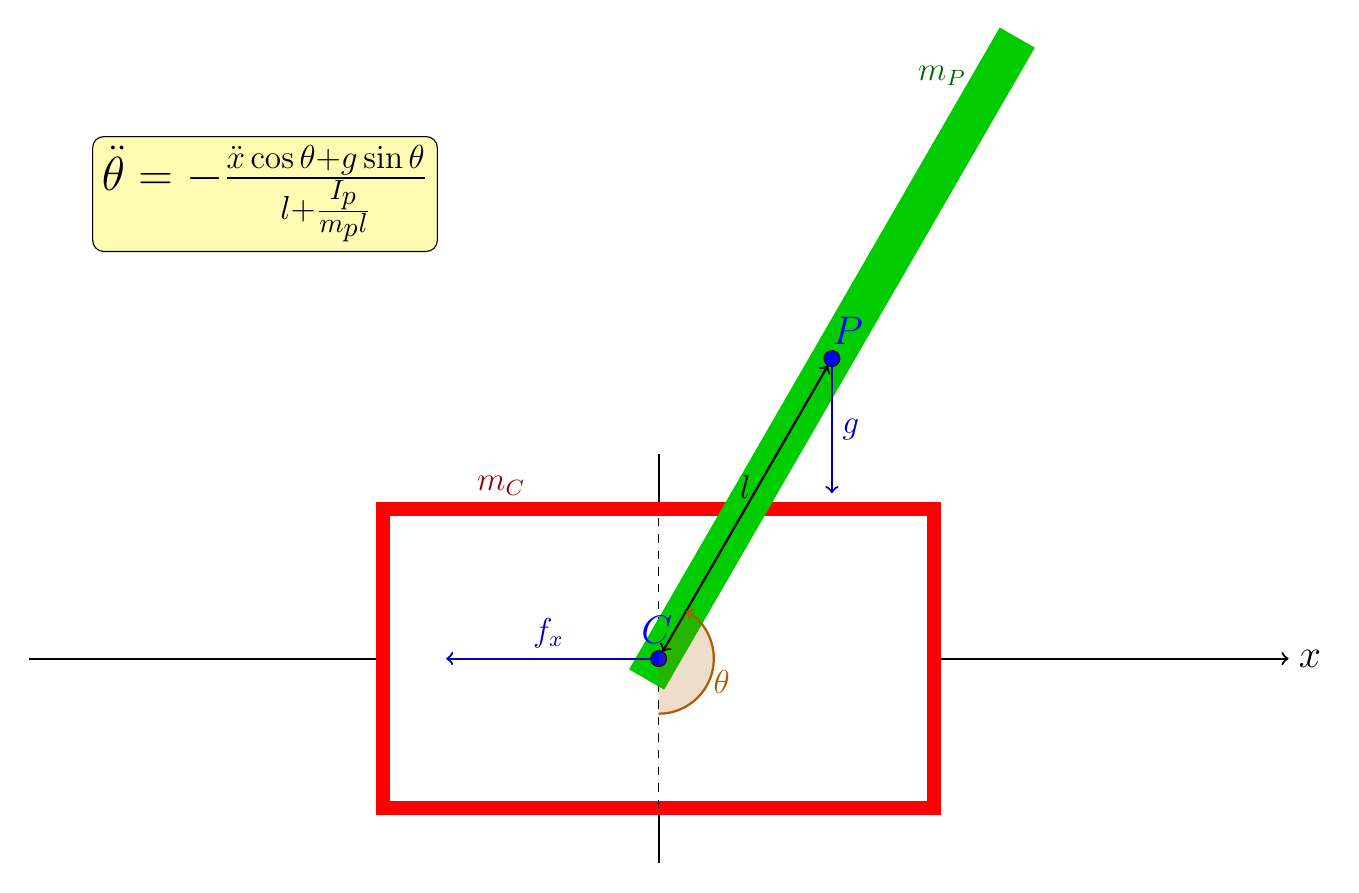
\begin{tikzpicture}
    % world
    \draw[->, thick] (-1,3.1) -- (15,3.1) node[right] {\Large $x$};
    \draw[-, thick] (7,0.5) -- (7,5.7);

    % hull
    \filldraw[red!100!black, fill=white, line width=5] (3.5,1.2) rectangle (10.5,5.0);

    % y axis help
    \draw[-, dashed] (7,1.2) -- (7,5.0);

    % stick
    \begin{scope}[rotate around={150:(7, 3.1)}]
        \filldraw[green!80!black, fill=green!80!black] (6.75, 3.4) rectangle (7.25, -6);

        % C
        \filldraw[fill=blue] (7, 3.1) circle [radius=0.1];
        \draw[blue] (7.2, 2.8) node {\Large $C$};

        % P
        \filldraw[fill=blue] (7, -1.3) circle [radius=0.1];
        \draw[blue] (7, -1.7) node {\Large $P$};

        % l
        \draw[<->, thick, black] (7,3) -- (7, -1.2) node[midway,above] {\large $l$};
    \end{scope}

    % f_x
    \draw[<-, thick, blue!70!black] (4.3,3.1) -- (6.9, 3.1) node[midway,above] {\large $f_x$};

    % g
    \draw[->, thick, blue!70!black] (9.2, 6.81) -- (9.2, 5.2) node[midway,right] {\large $g$};

    % \theta
    \draw[->, thick, orange!70!black] (7, 2.4) arc [start angle=-90, end angle=60, radius=0.7];
    \fill[->, opacity=0.2, orange!70!black] (7, 3.1) -- (7, 2.4) arc [start angle=-90, end angle=60, radius=0.7];
    \draw[thick, orange!70!black] (7.8, 2.8) node {\large $\theta$};

    % m_C
    \draw[red!60!black] (5, 5.3) node {\large $m_C$};

    % m_P
    \draw[green!40!black] (10.6, 10.5) node {\large $m_P$};

    % formula
    \draw (2,9) node[fill=yellow!30, draw, rounded corners] {\LARGE $\ddot{\theta} = - \frac{\ddot{x} \cos \theta + g \sin \theta}{l + \frac{I_p}{m_pl}}$};
\end{tikzpicture}
\end{document}
\end{center}

Coordinates of points and their derivatives
\begin{align*}
    & C = \pmat{x                 \\ 0};  & &\dot{C} = \pmat{\dot{x} \\ 0}; \\
    & P = \pmat{x + l \sin \theta \\ - l \cos \theta}; & &\dot{P} = \pmat{\dot{x} + l \dot{\theta} \cos \theta \\ l \dot{\theta} \sin \theta};
\end{align*}

Then the kinetic energy of the carriage is
\[
    T_C = \frac{1}{2} m_c \begin{Vmatrix}
        \dot{C}
    \end{Vmatrix}_2^2 = \frac{1}{2} m_c \dot{x}^2
\]


Kinetic energy of the pendulum
\begin{align*}
    T_p & = T^t_p + T^r_p =                                                                                                                             \\
        & = \frac{1}{2} m_p \begin{Vmatrix}\dot{P}\end{Vmatrix}_2^2 + \frac{1}{2}I_p\dot{\theta}^2 =                                                              \\
        & = \frac{1}{2} m_p (\dot{x} + l \dot{\theta} \cos \theta )^2 + \frac{1}{2} m_p (l \dot{\theta} \sin \theta)^2 + \frac{1}{2}I_p\dot{\theta}^2 = \\
        & = \frac{1}{2} m_p \dot{x}^2 + m_p \dot{x} l \dot{\theta} \cos \theta + \frac{1}{2} \dot{\theta}^2 \left( m_p l^2  + I_p \right)               \\
\end{align*}

Then the kinetic and potential energy of the whole system
\begin{align*}
    T & = T_c + T_p =                                                                                                                                               \\
      & = \frac{1}{2} m_c \dot{x}^2 + \frac{1}{2} m_p \dot{x}^2 + m_p \dot{x} l \dot{\theta} \cos \theta + \frac{1}{2} \dot{\theta}^2 \left( m_p l^2  + I_p \right) \\
      & = \frac{1}{2} \dot{x}^2 (m_c + m_p) + m_p \dot{x} l \dot{\theta} \cos \theta + \frac{1}{2} \dot{\theta}^2 \left( m_p l^2  + I_p \right)                     \\
      &                                                                                                                                                             \\
    U & = \underbrace{U_c}_{0} + U_p = -m_p gl \cos \theta                                                                                                          \\
\end{align*}

To calculate the dynamics of the system we will use the Euler-Lagrange differential equation
\[
    \frac{d}{dt} \frac{dL}{d\dot{q}} - \frac{dL}{dq} = Q
\]
where \( L = T - U \), \(Q\) is the generalized force and \(q = \pmat{x \\ \theta}\). From this we derive the equation of motion

\[
    \begin{cases}
        m_p \ddot{x} l \cos \theta + \ddot{\theta} \left(m_p l^2 + I_p\right) + m_p g l \sin \theta = 0  \\
        \ddot{x}(m_c + m_p) + m_p l \ddot{\theta} \cos \theta - m_p l \dot{\theta}^2 \sin \theta = f_{x}
    \end{cases}
\]

A more detailed calculation is below

\[
    L = \frac{1}{2} \dot{x}^2 (m_c + m_p) + m_p \dot{x} l \dot{\theta} \cos \theta + \frac{1}{2} \dot{\theta}^2 \left( m_p l^2  + I_p \right) + m_p gl \cos \theta
\]

\begin{align*}
    \frac{dL}{d\theta}                                         & = - m_p \dot{x} l \dot{\theta} \sin \theta - m_p gl \sin \theta                                                                                                                    \\
    \frac{dL}{d\dot{\theta}}                                   & = m_p \dot{x} l \cos \theta + \dot{\theta} \left(m_p l^2 + I_p\right)                                                                                                              \\
    \frac{d}{dt} \frac{dL}{d\dot{\theta}}                      & = m_p \ddot{x} l \cos \theta - m_p  \dot{x}  l \dot{\theta} \sin \theta + \ddot{\theta} \left(m_p l^2 + I_p\right)                                                                 \\
    \frac{d}{dt} \frac{dL}{d\dot{\theta}} - \frac{dL}{d\theta} & = m_p \ddot{x} l \cos \theta - m_p  \dot{x}  l \dot{\theta} \sin \theta + \ddot{\theta} \left(m_p l^2 + I_p\right) + m_p \dot{x} l \dot{\theta} \sin \theta + m_p gl \sin \theta = \\
                                                               & = m_p \ddot{x} l \cos \theta + \ddot{\theta} \left(m_p l^2 + I_p\right) + m_p g l \sin \theta                                                                                      \\
                                                               &                                                                                                                                                                                    \\
    \frac{dL}{dx}                                              & = 0                                                                                                                                                                                \\
    \frac{dL}{d\dot{x}}                                        & = \dot{x}(m_c + m_p) + m_p l \dot{\theta} \cos \theta                                                                                                                              \\
    \frac{d}{dt} \frac{dL}{d\dot{x}}                           & = \ddot{x}(m_c + m_p) + m_p l \ddot{\theta} \cos \theta - m_p l \dot{\theta}^2 \sin \theta                                                                                         \\
    \frac{d}{dt} \frac{dL}{d\dot{x}} - \frac{dL}{dx}           & = \ddot{x}(m_c + m_p) + m_p l \ddot{\theta} \cos \theta - m_p l \dot{\theta}^2 \sin \theta                                                                                         \\
\end{align*}

\subsection{Controlling acceleration}

Convert the second equation in the resulting system

\[
    \begin{cases}
        m_p \ddot{x} l \cos \theta + \ddot{\theta} \left(m_p l^2 + I_p\right) + m_p g l \sin \theta = 0          \\
        \ddot{x}  = \frac{f_{x} - m_p l \ddot{\theta} \cos \theta + m_p l \dot{\theta}^2 \sin \theta}{m_c + m_p}
    \end{cases}
\]

Consider that we can obtain any such \(f_x\) at any time that \(\ddot{x}\) can take any value from \([-a, a]\). Then the second equality does not make sense further, instead we can consider the first one

\[
    m_p \ddot{x} l \cos \theta + \ddot{\theta} \left(m_p l^2 + I_p\right) + m_p g l \sin \theta = 0
\]
\[
    \ddot{\theta} = - \frac{m_p \ddot{x} l \cos \theta + m_p g l \sin \theta}{m_p l^2 + I_p} = - \frac{\ddot{x} \cos \theta + g \sin \theta}{l + \frac{I_p}{m_pl}}
\]

It turns out that the equation of motion is described by this equation, where \(\ddot{x}\) is given by any in the segment \([-a, a]\).

\subsection{Friction}
The friction affecting \(\ddot{x}\) is not considered, since it is given by any number from the segment \([-a, a]\). One can introduce friction on \(\ddot{\theta}\) of the general form \(f(\theta, \dot{\theta})\) (for example, linear from angular velocity \(f(\theta, \dot{\theta}) = \mu \dot{\theta}\), where \(\mu\) is a constant), then the equation of motion rewrites as
\[
    \ddot{\theta} = - \frac{\ddot{x} \cos \theta + g \sin \theta}{l + \frac{I_p}{m_pl}} + f(\theta, \dot{\theta})
\]

\newpage
\section{Radial Cart Pole}

\begin{center}
    \documentclass[dvisvgm,tikz]{standalone}

\usepackage{amsmath}
\usepackage{mathpazo}
\usepackage[utf8]{inputenc}
\usepackage{graphics}
\usepackage[colorlinks,urlcolor=blue]{hyperref}
\usepackage{standalone}
\usepackage{svg}
\usepackage{tikz}
\usepackage{tikz-3dplot}

\usetikzlibrary{arrows.meta,decorations.pathreplacing,calligraphy}

\usetikzlibrary{arrows.meta}
\special{background White}

\begin{document}
% camera params
\tdplotsetmaincoords{70}{110}

\begin{tikzpicture}[tdplot_main_coords, scale = 10, >=stealth]
    % EPSILON
    \pgfmathsetmacro{\e}{0.001}

    % rotate sticks params
    \pgfmathsetmacro{\alpha}{-30}
    \pgfmathsetmacro{\beta}{-40}

    % first stick params
    \pgfmathsetmacro{\a}{0.8}
    \pgfmathsetmacro{\aext}{0.1}
    \pgfmathsetmacro{\phirad}{0.15}

    % second stick params
    \pgfmathsetmacro{\b}{0.5}
    \pgfmathsetmacro{\bext}{0.1}
    \pgfmathsetmacro{\thetarad}{0.08}

    % right angles size
    \pgfmathsetmacro{\rs}{0.03}

    % world axis params
    \draw[->] (0,0,0) -- (1,0,0) node[anchor=north east]{\large $x$};
    \draw[->] (0,0,0) -- (0,1,0) node[anchor=north west]{\large $y$};
    \draw[->] (0,0,0) -- (0,0,0.7) node[anchor=south]{\large $z$};

    \draw[dashed, canvas is xy plane at z=0] (\a,0)  arc[start angle=0, end angle=90, radius=\a];

    \tdplotsetrotatedcoords{\alpha}{\beta}{0}
    \begin{scope}[tdplot_rotated_coords]
        % l_r
        \draw[pen colour={gray}, line width=0.8, decorate, decoration = {calligraphic brace, raise=5, amplitude=4}] (0, 0, 0.002) -- (0, {(\a - \aext)/2 - 0.02}, 0.002);
        \draw[gray] (0, {(\a - \aext)/4}, 0.06) node {$l_r$};

        % r
        \draw[pen colour={gray}, line width=0.8, decorate, decoration = {calligraphic brace, raise=5, amplitude=4}]  (0, {\a - 0.02}, -0.002) -- (0, 0, -0.002);
        \draw[gray] (0, \a / 2, -0.06) node {$r$};

        % l_p
        \draw[pen colour={gray}, line width=0.8, decorate, decoration = {calligraphic brace, raise=5, amplitude=4}] (0.02, \a, 0.01) -- (0.02, \a, {\b/2 - 0.01});
        \draw[gray] (0.09, \a, {\b/4 - 0.01}) node {$l_p$};

        % red stick
        \draw[line width=3, color=red!100!black] (0, -\aext, 0) -- (0, \a, 0);
        \path[canvas is zx plane at y={(\a-\aext)/2}] (0,0,0) node[color=blue, circle, fill, inner sep=2]{};
        \draw[blue, canvas is zx plane at y={(\a-\aext)/2}] (0.04, -0.02) node {\Large $R$};

        % green stick
        \draw[line width=3, color=green!80!black] (0, \a, -\bext) -- (0, \a, \b+\bext);
        \path[canvas is zx plane at y=\a] ({\b/2},0) node[color=blue, circle, fill, inner sep=2]{};
        \draw[blue, canvas is zx plane at y=\a] ({\b/2 + 0.01}, 0.03) node {\Large $P$};

        % theta angle
        \draw[<-, thick, orange!70!black, canvas is zx plane at y=\a] (\thetarad, 0) arc [start angle=0, end angle=-180-\beta, radius=\thetarad];
        \fill[<-, orange!70!black, opacity=0.2, canvas is zx plane at y=\a] (0, 0) -- (\thetarad, 0) arc [start angle=0, end angle=-180-\beta, radius=\thetarad];
        \draw[dashed, canvas is zx plane at y=\a] (-180-\beta:0) -- (-180-\beta:\thetarad);
        \draw[canvas is zx plane at y=\a, orange!70!black] ({(-180-\beta)/2}:\thetarad+0.02) node {$\theta$};

        % red-green right angle
        \draw[canvas is yz plane at x=0] (\a-\rs,0) -- (\a-\rs,\rs) -- (\a, \rs);

        % green right angle
        \draw[canvas is zx plane at y=\a] (-180-\beta:\rs) -- (-135-\beta:{sqrt(2)*\rs}) -- (-90-\beta:\rs);
    \end{scope}

    % phi angle
    \draw[->, thick, orange!70!black] (\phirad, 0) arc [start angle=0, end angle=90+\alpha, radius=\phirad];
    \fill[->, opacity=0.2, orange!70!black] (0, 0) -- (\phirad, 0) arc [start angle=0, end angle=90+\alpha, radius=\phirad];
    \draw[orange!70!black]  ({(80+\alpha)/2}:\phirad+0.05) node {$\phi$};

    % formula
    \draw (0.0,0.4,0.5) node[fill=yellow!30, draw, rounded corners] {\large $\ddot{\theta} = - b\dot{\theta} - k \big( \ddot{\phi} r \cos \theta + g\sin \theta \big) $};
    \draw (0.0,0.21,0.35) node[fill=yellow!30, draw, rounded corners] {\large $\ddot{\phi} = u$};
\end{tikzpicture}
\end{document}

\end{center}

In this problem, too, we consider that we control \(\ddot{\phi}\) instead of \(f_{\phi}\) at once, which means that the Euler-Lagrange can be derived only by the coordinate \(\theta\)

\[
    \frac{d}{dt} \frac{dL}{d\dot{\theta}} - \frac{dL}{d\theta} = 0
\]

After calculating all the components we obtain the equation

\[
    \ddot{\theta} = - \frac{\ddot{\phi} r \cos \theta + g\sin \theta}{l_p + \frac{I_p}{m_p l_p}}
\]

A more detailed calculation

\[
    T_r = \frac{1}{2}\dot{\phi}^2(I_r + m_rl_r^2)
\]
\[
    T_p = T_p^t + T_p^c
\]

Note that \(T_p^c = \frac{1}{2}I_p\dot{\theta}^2\) and \(T_p^t = \frac{1}{2}m_p\begin{Vmatrix} \dot{P} \end{Vmatrix}_2^2\). To calculate \(\begin{Vmatrix} \dot{P} \end{Vmatrix}_2^2\), consider the system with respect to the coordinate system in the figure below
\begin{center}
    \documentclass[dvisvgm,tikz]{standalone}
 
\usepackage{amsmath}
\usepackage{mathpazo}
\usepackage[utf8]{inputenc}
\usepackage{graphics}
\usepackage[colorlinks,urlcolor=blue]{hyperref}
\usepackage{standalone}
\usepackage{svg}
\usepackage{tikz}
\usepackage{tikz-3dplot}

\usetikzlibrary{arrows.meta,decorations.pathreplacing,calligraphy}
\special{background White}

\begin{document}
% camera params
\tdplotsetmaincoords{70}{110}
 
\begin{tikzpicture}[tdplot_main_coords, scale = 10, >=stealth]
    % EPSILON
    \pgfmathsetmacro{\e}{0.001}
 
    % rotate sticks params
    \pgfmathsetmacro{\alpha}{-30}
    \pgfmathsetmacro{\beta}{-40}
 
    % first stick params
    \pgfmathsetmacro{\a}{0.8}
    \pgfmathsetmacro{\aext}{0.1}
    \pgfmathsetmacro{\phirad}{0.15}
 
    % second stick params
    \pgfmathsetmacro{\b}{0.5}
    \pgfmathsetmacro{\bext}{0.1}
    \pgfmathsetmacro{\thetarad}{0.08}
 
    % right angles size
    \pgfmathsetmacro{\rs}{0.03}
 
    % world axis params
    \draw[-] (0,0,0) -- (1,0,0);
    \draw[-] (0,0,0) -- (0,1,0);
    \draw[-] (0,0,0) -- (0,0,0.4);
 
    \draw[dashed, canvas is xy plane at z=0] (\a,0)  arc[start angle=0, end angle=90, radius=\a];
 
    \tdplotsetrotatedcoords{\alpha}{\beta}{0}
    \begin{scope}[tdplot_rotated_coords]
        % red stick
        \draw[line width=3, color=red!100!black] (0, -\aext, 0) -- (0, \a, 0);
        \path[canvas is zx plane at y={(\a-\aext)/2}] (0,0,0) node[color=blue, circle, fill, inner sep=2]{};
        \draw[blue, canvas is zx plane at y={(\a-\aext)/2}] (0.04, -0.02) node {\Large \(R\)};
 
        % green stick
        \draw[line width=3, color=green!80!black] (0, \a, -\bext) -- (0, \a, \b+\bext);
        \path[canvas is zx plane at y=\a] ({\b/2},0) node[color=blue, circle, fill, inner sep=2]{};
        \draw[blue, canvas is zx plane at y=\a] ({\b/2 + 0.01}, 0.03) node {\Large \(P\)};
     \end{scope}
 
    % axes
    \tdplotsetrotatedcoords{\alpha}{0}{0}
    \begin{scope}[tdplot_rotated_coords]
        % x'
        \draw[->, canvas is xz plane at y=\a] (0.2, 0) -- (-0.2, 0) node[anchor= west]{$x'$};
 
        % y'
        \draw[->, canvas is xz plane at y=\a] (0, -0.2) -- (0, 0.2) node[anchor= west]{$y'$};
    \end{scope}
 
    % phi angle
    \draw[->, thick, orange!70!black] (\phirad, 0) arc [start angle=0, end angle=90+\alpha, radius=\phirad];
    \fill[->, opacity=0.2, orange!70!black] (0, 0) -- (\phirad, 0) arc [start angle=0, end angle=90+\alpha, radius=\phirad];
    \draw[orange!70!black]  ({(80+\alpha)/2}:\phirad+0.05) node {\(\phi\)};
 \end{tikzpicture}
\end{document}

\end{center}
velocity \(\begin{Vmatrix} \dot{P} \end{Vmatrix}_2^2\) is decomposed by the coordinates \(y\) and \(z\), we get that
\[
    \begin{Vmatrix} \dot{P} \end{Vmatrix}_2^2 = \left(\underbrace{\dot{\phi} r + \dot{\theta} l_p \cos \theta }_{\dot{y}}\right)^2 + \left(\underbrace{\dot{\theta} l_p \sin \theta}_{\dot{z}} \right)^2 = \dot{\phi}^2 r^2 + 2 \dot{\phi} \dot{\theta} r l_p \cos \theta + \dot{\theta}^2 l_p^2
\]

It remains to do the trivial calculations
\[
    T_p = \frac{1}{2}I_p\dot{\theta}^2 + \frac{1}{2}m_p\left(\dot{\phi}^2 r^2 + 2 \dot{\phi} \dot{\theta} r l_p \cos \theta + \dot{\theta}^2 l_p^2\right)
\]
\[
    T = T_r + T_p = \frac{1}{2}\dot{\phi}^2(I_r + m_rl_r^2) + \frac{1}{2}I_p\dot{\theta}^2 + \frac{1}{2}m_p\left(\dot{\phi}^2 r^2 + 2 \dot{\phi} \dot{\theta} r l_p \cos \theta + \dot{\theta}^2 l_p^2\right)
\]
\[
    U = \left( \underbrace{U_r}_{0} + U_p \right) = - m_p g l_p \cos \theta
\]
\[
    L = T - U = \frac{1}{2}\dot{\phi}^2(I_r + m_rl_r^2) + \frac{1}{2} I_p \dot{\theta}^2 + \frac{1}{2} m_p \left(\dot{\phi}^2 r^2 + 2 \dot{\phi} \dot{\theta} r l_p \cos \theta + \dot{\theta}^2 l_p^2\right) + m_p g l_p \cos \theta
\]
\begin{align*}
    \frac{dL}{d\theta}                                         & = - m_p l_p (r \dot{\phi} \dot{\theta} \sin \theta + g \sin \theta)                                                   \\
    \frac{dL}{d\dot{\theta}}                                   & = I_p \dot{\theta} + m_p l_p (\dot{\phi} r \cos \theta + l_p \dot{\theta})                                            \\
    \frac{d}{dt} \frac{dL}{d\dot{\theta}}                      & = I_p \ddot{\theta} + m_p l_p (r \ddot{\phi} \cos \theta + l_p \ddot{\theta} - r \dot{\phi} \dot{\theta} \sin \theta) \\
    \frac{d}{dt} \frac{dL}{d\dot{\theta}} - \frac{dL}{d\theta} & =
    I_p \ddot{\theta} + m_p l_p (r \ddot{\phi} \cos \theta + l_p \ddot{\theta} - r \dot{\phi} \dot{\theta} \sin \theta) + m_p l_p (r \dot{\phi} \dot{\theta} \sin \theta + g \sin \theta) = \\
                                                               & = I_p \ddot{\theta} + m_p l_p (r \ddot{\phi} \cos \theta + l_p \ddot{\theta}) + m_p l_p g \sin \theta =               \\
                                                               & = \ddot{\theta} (I_p  + m_p l_p^2) + m_p l_p (r \ddot{\phi} \cos \theta + g \sin \theta) = 0
\end{align*}
\end{document}